\section{Method}
\subsection{Dataset}
We used both public dataset and customized dataset to train and evaluate our model.
Firstly, the MS-COCO~\cite{datasetcoco} which contains 2.5 million annotated 
instances in 328k images categorized as 91 types. As our aim is to train a model that 
can not only locate birds in images but also avoid false detections that recognize 
non-bird objects as birds. All 80 types of training subset is used. However, as 
the MS-COCO dataset is lack of instances of birds that is difficult to be detected.
We collected 708 birds image in field environment and manually labeled all these birds 
instances with their bounding boxes and segments. Many of these instances is hard to be 
detected because of factors such as occlusion. Besides, we also noted birds with the 
following criterias.
\begin{enumerate}
    \item whether the instance is occluded.
    \item whether the instance is not clear.
    \item whether the instance is photographed in side direction.
    \item whether the instance is photographed in backlighting condition.
\end{enumerate}
A tabel describing our dataset based on these four criterias is shown in~\ref{th-bird-table}.
\begin{table}[H]
    \centering  % 使表格居中
    \captionsetup{justification=centering}  % 使标题居中
    \begin{tabular}{|c|c|}
    \hline
                       & Instances amount \\ \hline
    Occluded           & 262              \\ \hline
    Not clear          & 400              \\ \hline
    Not side direction & 136              \\ \hline
    Backlighting       & 70               \\ \hline
    Total              & 1142             \\ \hline
    \end{tabular}
    \caption{Summary of TH-Bird dataset}
    \label{th-bird-table}
\end{table}
\subsection{Data augmentation}
In order to simulate a shooting scene in the field, 
we adapted and designed some data argument methods. 
In the existing method, we apply the random disorder 
in color zone, random horizontal flip, 
random crop and random extend.

In the field environment, birds may be occluded by 
branches or be unclear on photos because of movement. 
We designed the stochastic fuzzy algorithm and 
random occlusion algorithm to simulate. 
\subsubsection{Stochastic fuzzy algorithm}
Firstly, extract the bounding boxes coordinates of 
birds instances and determine the area to be blurred. 
Then, apply a convolution kernel of a specific size. 
All weights of this kernel is one. Therefore, the 
convolution results can be derived as 
\[
I'(x, y) = \sum_{i=-k}^{k} \sum_{j=-k}^{k} K(i, j) \cdot I(x+i, y+j)
\]
\begin{itemize}
    \item \( I(x, y) \): Original pixel value at \((x, y)\).
    \item \( I'(x, y) \): Blurred pixel value at \((x, y)\).
    \item \( K(i, j) \): Kernel value at \((i, j)\).
    \item \( k \): Half the kernel size (e.g., for a 3x3 kernel, \( k=1 \)).
\end{itemize}
For example, to get average value from 3X3 regions.
The weights are chosen as:
\[
K = \frac{1}{9}
\begin{bmatrix}
1 & 1 & 1 \\
1 & 1 & 1 \\
1 & 1 & 1
\end{bmatrix}
\]
\subsubsection{Random occlusion algorithm}
Being blocked by branches is a very common circumstances in 
bird photography. We design an algorithm to generate 
simulated branches from data augmentation. To obtain 
the optimized color, the RGB color and standard deviation
of each channel were counted in a branches dataset~\cite{datsetbr}.
The statistic results are shown in~\ref{bra-table}
\begin{table}[H]
    \centering  % 使表格居中
    \captionsetup{justification=centering}  % 使标题居
    \begin{tabular}{|c|c|c|}
    \hline
    \backslashbox{Value}{Channels}  & Average value & Standard deviation \\ \hline
    R & 87.35         & 2.487              \\ \hline
    G & 89.24         & 2.497              \\ \hline
    B & 82.97         & 2.435              \\ \hline
    \end{tabular}
    \caption{Average value and standard deviation from~\cite{datsetbr}}
    \label{bra-table}
\end{table}

\begin{figure}[H]
    \centering
    \begin{subfigure}{0.20\textwidth} % 每张图的宽度为容器宽度的45%
        \includegraphics[width=\linewidth]{AugSampleImages/1.png} % 替换为你的图片路径
    \end{subfigure}
    \begin{subfigure}{0.20\textwidth}
        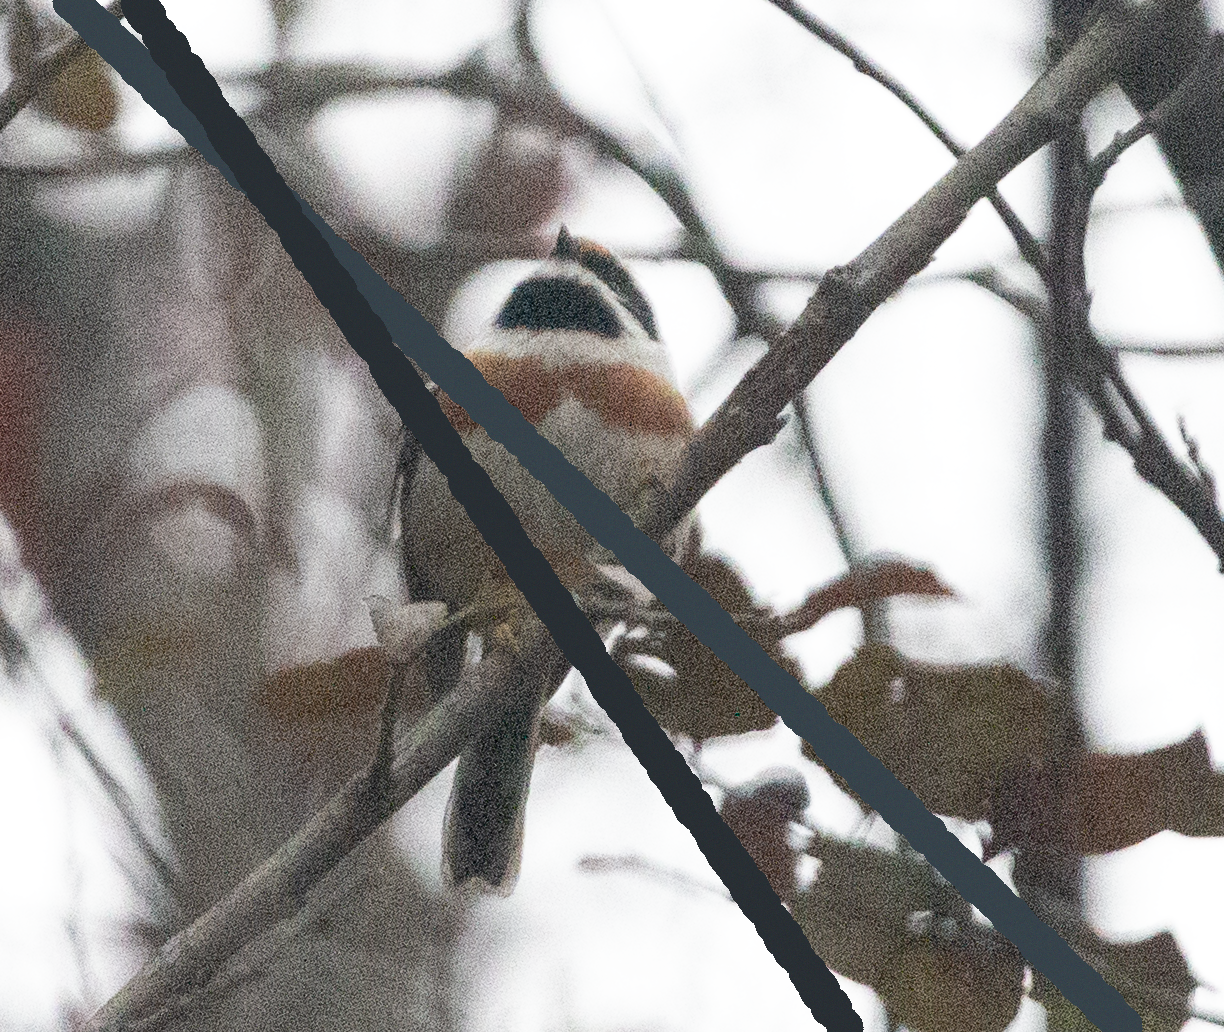
\includegraphics[width=\linewidth]{AugSampleImages/1X.png}
    \end{subfigure}

    \vspace{0.5em} % 行间距调整
    \begin{subfigure}{0.20\textwidth}
        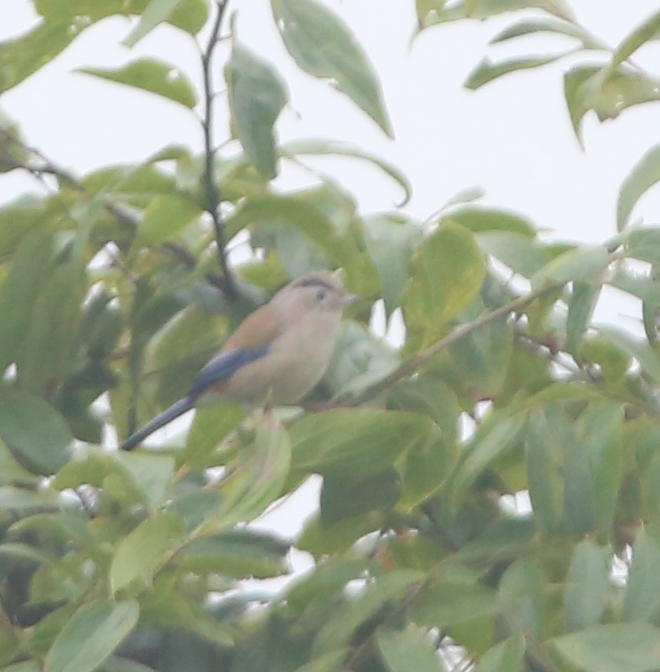
\includegraphics[width=\linewidth]{AugSampleImages/2.png}
    \end{subfigure}
    \begin{subfigure}{0.20\textwidth}
        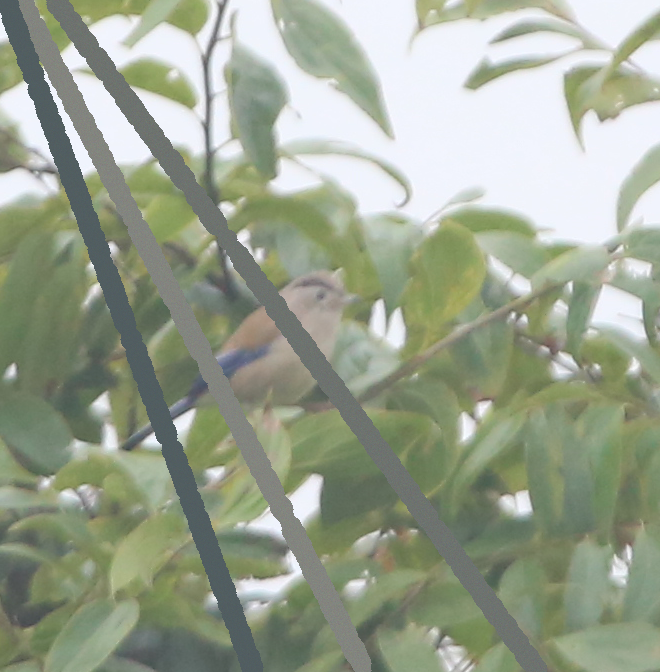
\includegraphics[width=\linewidth]{AugSampleImages/2X.png}
    \end{subfigure}

    \vspace{0.5em}
    \begin{subfigure}{0.20\textwidth}
        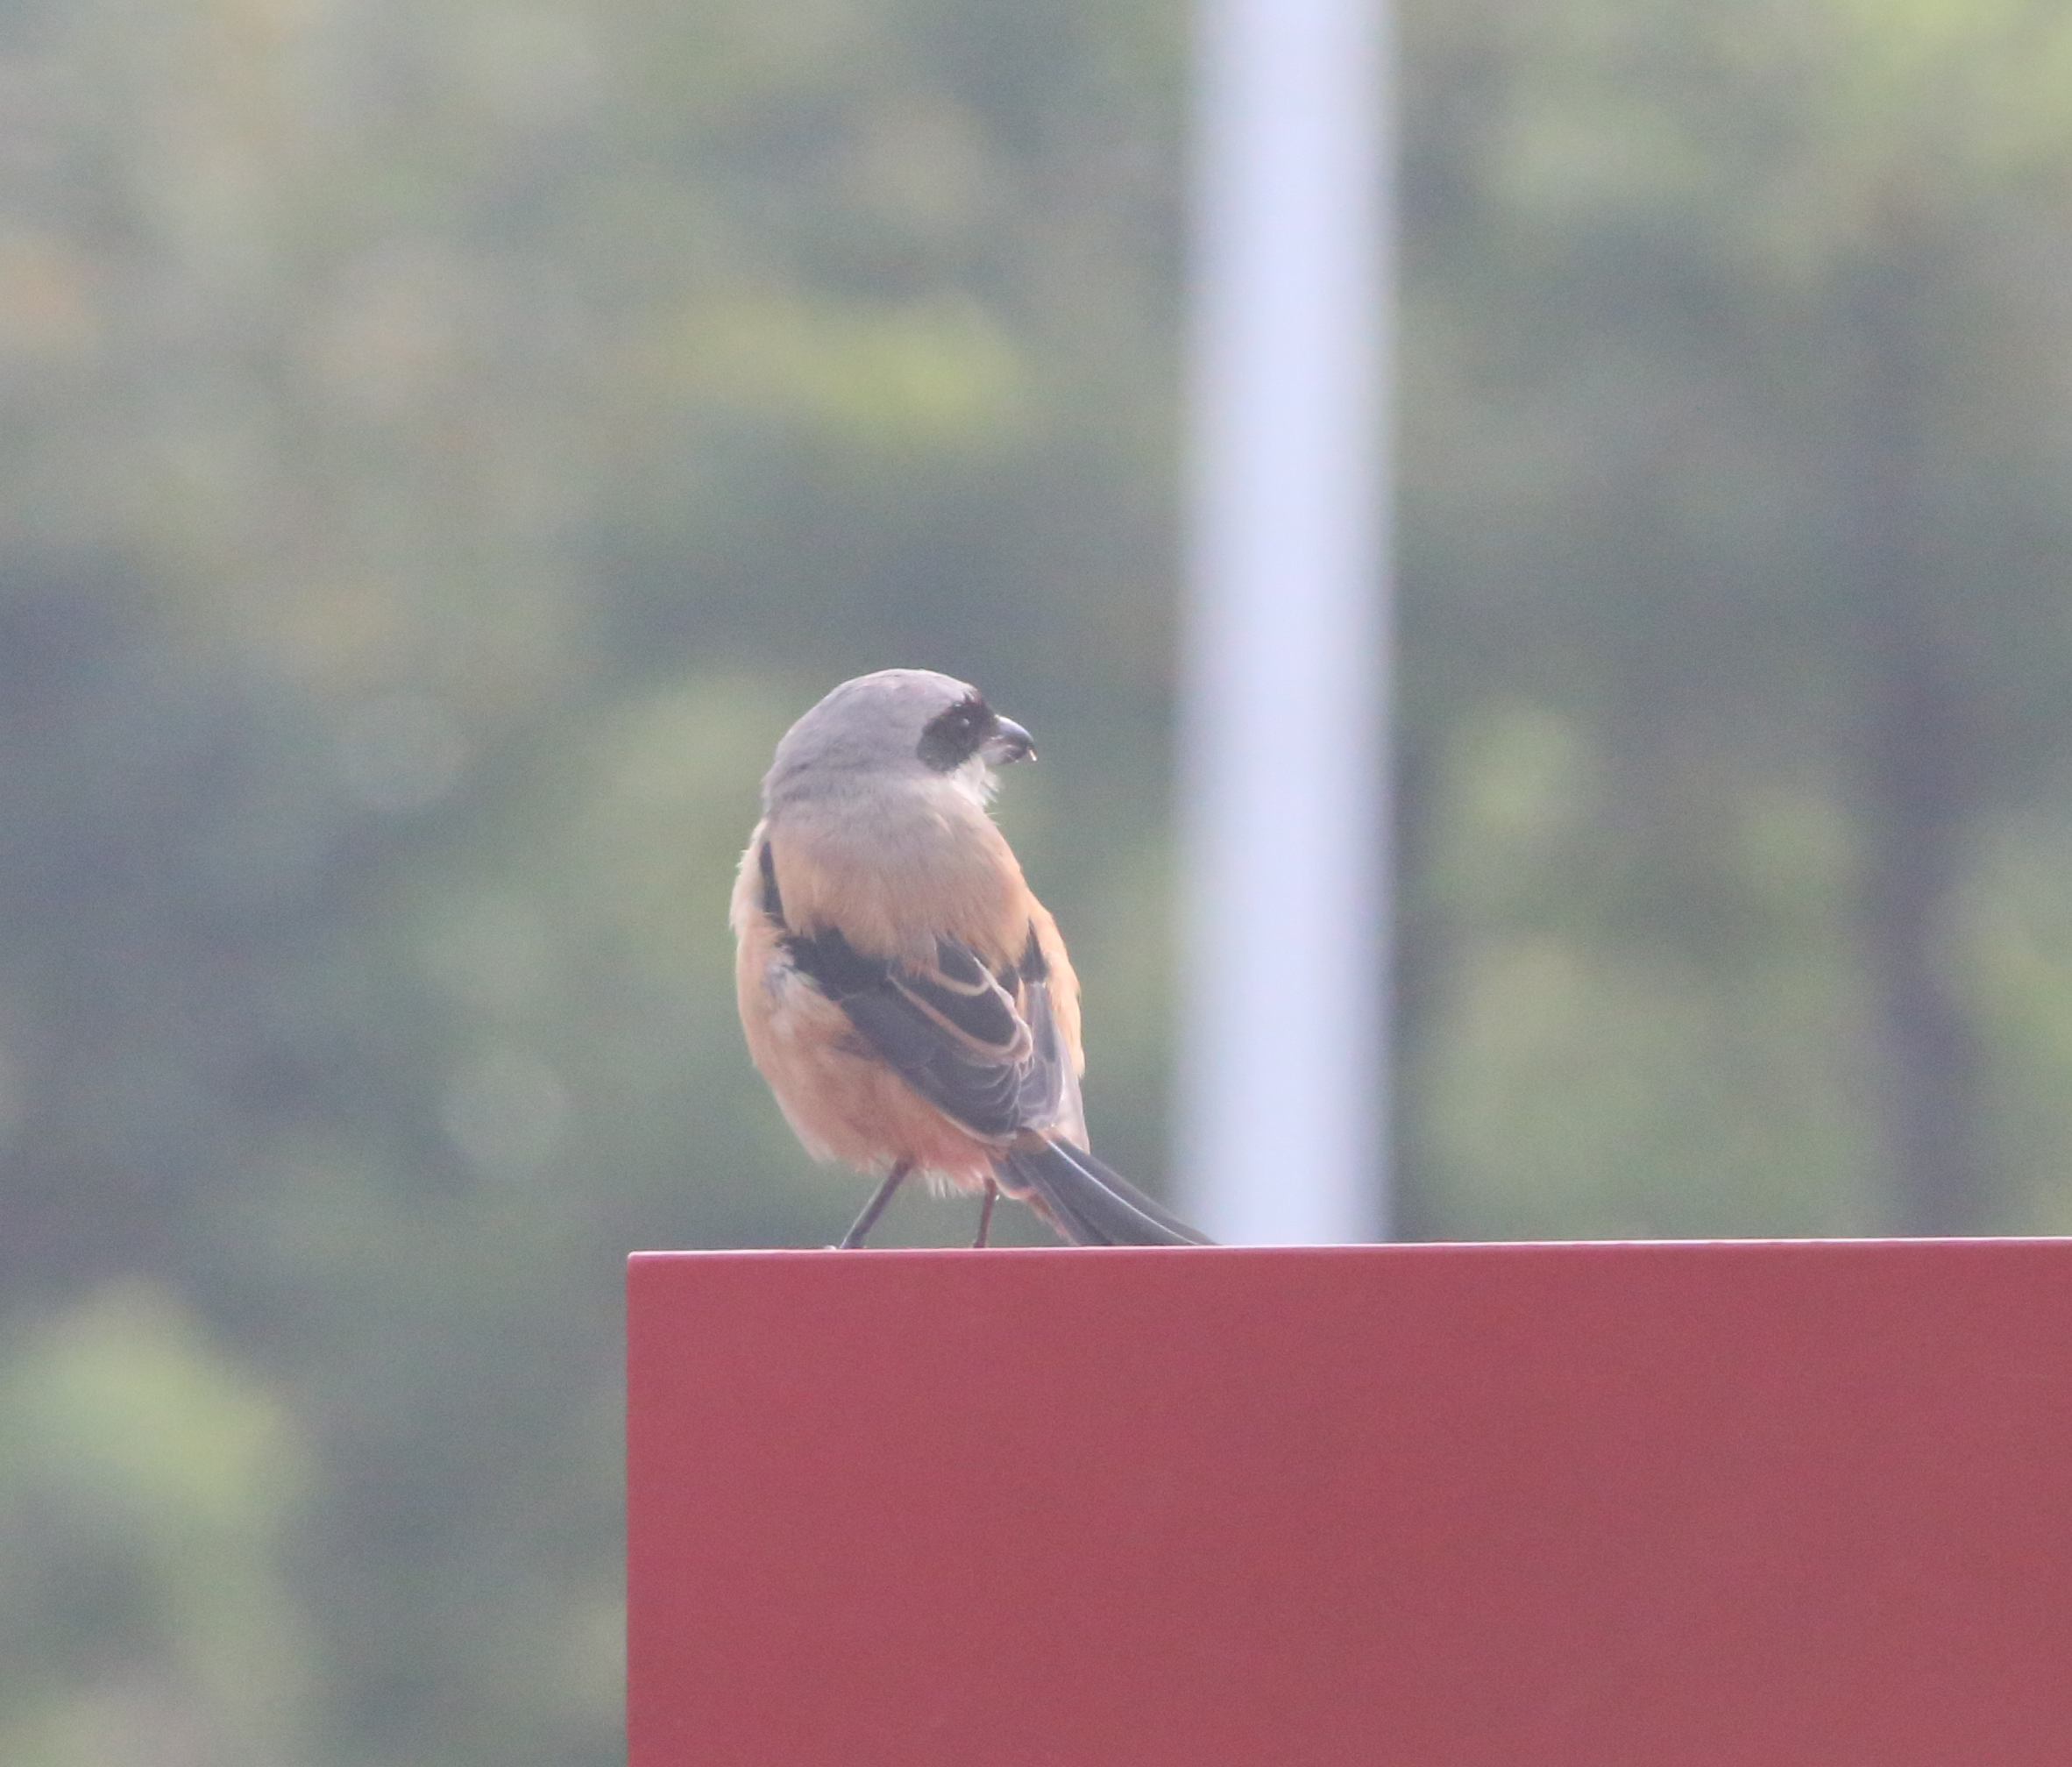
\includegraphics[width=\linewidth]{AugSampleImages/3.png}
    \end{subfigure}
    \begin{subfigure}{0.20\textwidth}
        \includegraphics[width=\linewidth]{AugSampleImages/3X.png}
    \end{subfigure}

    \vspace{0.5em}
    \begin{subfigure}{0.20\textwidth}
        \includegraphics[width=\linewidth]{AugSampleImages/4.png}
    \end{subfigure}
    \begin{subfigure}{0.20\textwidth}
        \includegraphics[width=\linewidth]{AugSampleImages/4X.png}
    \end{subfigure}
    
    \caption{Demonstrations of branches simulation algorithm}
    \label{aug-exp}
\end{figure}

The for each sample image, the birds instances 
are found and determine whether the bird's 
width and height are greater 25 to enable branches 
augmentation. To draw a occlusion line, its "center" point
is randomly selected within the bounding box. After that, 
the slope and x coordinates of the start and end points 
are determined. The y coordinates is derived with x coordinates,
slop and bonding box limit. The thinness varies along 
the line with an average value determined by the size of the 
bird and a fixed standard deviation. The flow graph and the pseudo 
code are displayed in 
